\documentclass[prb,preprint]{revtex4-1} 

\usepackage{amsmath}
\usepackage{amsfonts}
\usepackage{graphicx}

\begin{document}

\title{A confirmation of the Rydberg Constant and Mercury's Orbital  using }

\author{Ryan S. Morshead}

\affiliation{Department of Physics, California State Polytechnic University...}

\date{\today}

\begin{abstract}
Hydrogen and mercury discharge tubes are attached to a current source that will energize the atoms in the tube.  By passing ejected photons through a diffraction grating of known width and analyzing the magnitude of their diffraction one can find the wavelength of the photons being emitted and thus their energies. With these measurements for mercury's spectrum, the known energies corresponding to the transitions 6s6d 6$^3$P$_1\rightarrow$6s6p 6$^1$P$_1$, 6s6d 6$^3$D$_2\rightarrow$6s6p 6$^1$P$_1$, 6s7s 7$^3$S$_1\rightarrow$6s6p 6$^3$P$_2$, 6s7s 7$^3$S$_1\rightarrow$6s6p 6$^3$P$_1$, and 6s8s 8$^1$S$_0\rightarrow$6s6p 6$^1$P$_1$ were found to be in agreement with this experiment's findings for the energies of  $2.15\pm0.01$ eV, $2.17\pm0.01$ eV, $2.28\pm0.01$ eV, $2.85\pm0.07$ eV, and $2.53\pm0.01$ eV respectively. In addition, with the knowledge that the spectral lines of hydrogen which were measured, arise from the Balmer series, The Rydberg's Equation can be used to associate changes in the orbital energy of electrons and the wavelength of the photons being emitted. By the requirements of that association, the experiment described in this paper reports The Rydberg Constant to be $13.5\pm0.10$ eV. This measurement is in agreement with the officially determined value of 13.6 eV.



\end{abstract}


\maketitle

\section{Introduction}
The early 20\textsuperscript{th} century brought about experiments by Ernest Rutherford and Joseph Thomson which strongly established that atoms were made of a diffuse cloud of negatively charged electrons and some positive component. However the theories which hoped to describe the laws governing the atomic system had serious problems. In 1911 Rutherford's theory of atomic structure had recently dethroned Thomson's ``plumb pudding model" following the results from Rutherford's gold foil experiment \cite{geiger}. The Rutherford Model proposed that atoms were composed of a very small nucleus of high positive charge and a set of small negatively charged particles called electrons which orbited in the electric field created by the nucleus \cite{ruth}. However this model did not attribute any further structure to the electrons. Thus, because in this description, the electrons were only bound by an electric field, atoms would be inherently unstable; outside influences could easily cause electrons to spiral in and collide with the positively charged nucleus emitting a stream of photons with continuously increasing wavelength until that point. This posed large problems for the theory as atoms are clearly not unstable in the manner it described and atomic emissions were in fact found to be discrete. Rutherford's model was eventually replaced by Niels Bohr's model of the atom which, though not entirely explanatory of all atomic structures, nearly perfectly explained what had been observed concerning hydrogen. By adapting Rutherford's nuclear structure to fit Max Planck's quantum theory, Bohr introduced the idea that the chemical properties of each element were largely determined by the number of electrons in the outer orbits of its atoms \cite{bohr1,bohr2,bohr3}. He also introduced the idea that the orbital radii of electrons were discrete and that electrons could drop from higher-energy orbits to lower ones emitting energy in quanta in the process \cite{bohr1,bohr2,bohr3}.

The work done in this experiment looks to measure Johannes Rydberg's constant which relates the differences in orbital energies and the wavelengths of the corresponding photons in the hydrogen atom. In relation to mercury it seeks to confirm the energies of photons predicted by modern quantum atomic models and to see that the measurements made by this experiment agree with their current accepted values determined by other studies.

\newpage
\section{Experimental Design}
\subsection{Hydrogen}
To conduct the following experiment, an optical grating spectrometer is used in order to diffract incoming light and measure the angle of the diffraction. Hydrogen and mercury discharge tubes are used as light sources. The first thing that must be done is ensure that any light passing through either the collection tube or the viewing tube is collimated. this is done through autocollimation, where parallel rays of light leave an optical system and are reflected back into the same system by a plane mirror. This ensures that the image being carried by the light and can be focused sharply on a desired point by a movable lens in the tube. this is done for both the viewing tube and the collection tube where the image is focused from the slit, and on the crosshairs in the respective viewing tube. Shown in Figure \ref{ExpFig} is the case for measuring a negative diffraction angle. Because the image is mirrored on both sides of the of the zero line, making measurements of both, and then averaging them will minimize error arising from slight offsets in the diffraction grating.

\begin{figure}[h]
\centering
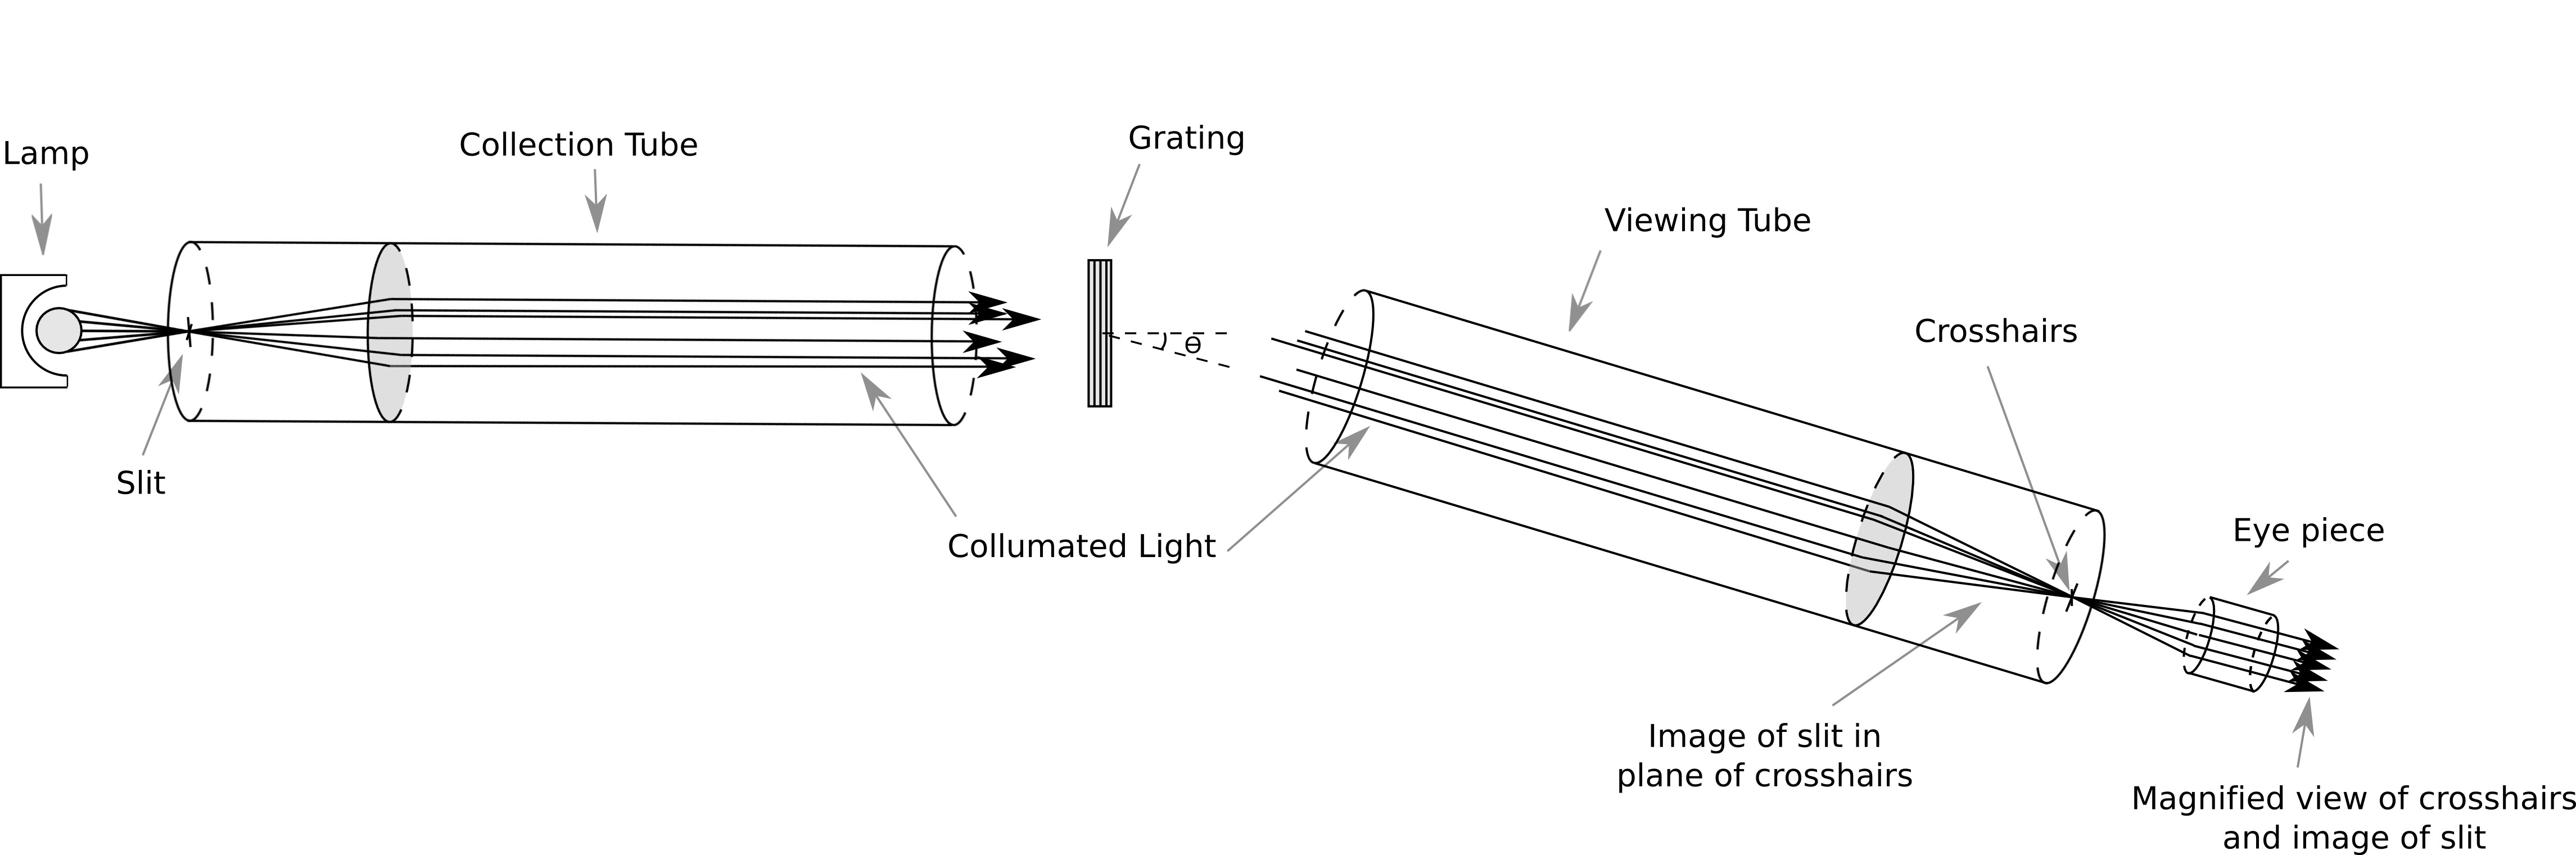
\includegraphics[width=\textwidth]{Lab2Fig.png}
\caption{Optical grating spectrometer in the case of viewing a negative diffraction angle}
\label{ExpFig}
\end{figure}

The collimated light which passes through the grating, whose slit widths are of a length $d$, will be diffracted to an angle $\theta$. By measuring $\theta$ for the first order diffraction, Eq. \eqref{eq1} can be used to determine the wavelength ($\lambda$) of light which passed through the grating.

\begin{equation}
n \lambda = d sin(\theta),
\label{eq1}
\end{equation}

By choosing to measure $\theta$'s for first order diffractions $n=1$. Knowing that the observed spectral lines from hydrogen arise from the Balmer series, in which electrons drop from higher energy orbitals to the second level orbital, Rydberg's equation, expressed in Eq. \eqref{eq2}, can be used to relate the corresponding changes in orbital energy to the energy released by photons in that process. As a result, the Rydberg Constant ($E_R$) must, by that association, carry a particular value to link the two.

\begin{equation}
E_{\gamma}=\frac{hc}{\lambda}=E_R\left(\frac{1}{n'^2}-\frac{1}{n^2}\right) ,
\label{eq2}
\end{equation}

By using emission lines from the Balmer series $n'=2$. This relationship can then be manipulated to fit the form $y=mx+b$ where $y=\lambda$, $(hc)/E_R=m$, and the remaining term is equal to $x$. the resulting form is shown by Eq. \eqref{eq:eq3}.

\begin{equation}
\lambda=\frac{hc}{E_R}\left(\frac{1}{2^2}-\frac{1}{n^2}\right)^{-1}.
\label{eq:eq3}
\end{equation}

In this form, data from the wavelengths of the observed spectrum can be used in tandem with the corresponding orbital potentials to perform a least squares optimization of the value $m$ and the $y$-intercept, $b$.

\subsection{Mercury}

Determining the diffraction angles for mercury requires the same apparatus shown in Fig. \ref{ExpFig}, and method of measurement used to determine the diffraction angles for hydrogen. Thus following the collection of $\theta$ values, they are related to the wavelength of emitted light using Eq. \eqref{eq1} and then converted into energies using Eq. \eqref{finaleq}.

\begin{equation}
E_{\gamma}=\frac{hc}{\lambda}.
\label{finaleq}
\end{equation}

However this data is not fit to a linear curve because The Bohr Model and consequently The Rydberg Equation, do not accurately describe the emission spectra of heavier elements. As a result this experiment simply seeks to identify the energy transitions predicted by the standard model.
\newpage

\section{Results and Analysis}
\subsection{Hydrogen}
With $\lambda$ data collected from the optical grating spectrometer a least squares optimization of Eq. \eqref{eq:eq3} was used to find the value of $(hc)/E_R$ which best fit the data. Then, by removing a factor of $hc$ from the optimized value for m, a calculated value for $E_R$ is output. The final results for $\theta$, $\lambda$, and the corresponding energies ($E_\gamma$) are shown by Table \ref{STUFF}. The linear curve fit for Eq. \eqref{eq:eq3} is shown by Fig \ref{linfit}.

\begin{figure}[h]
\centering
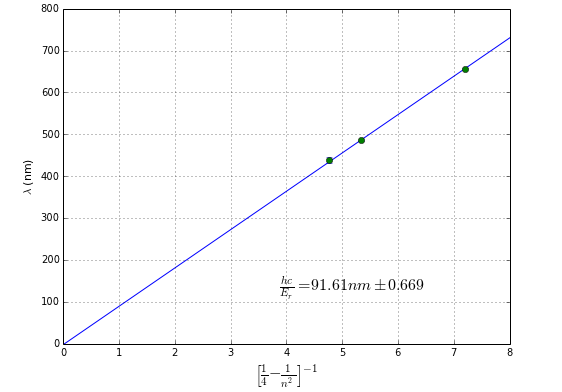
\includegraphics[width=\textwidth]{linfit.png}
\caption{Least squares curve fit of wavelength data and the corresponding initial orbital potential with calculated value of the slope.}
\label{linfit}
\end{figure}

\begin{table}[h!]
\caption{Final values for $E_\gamma$ and other pertinent data associated with hydrogen}
\begin{ruledtabular}
\begin{tabular}{r c c c p{4 cm}}
$\theta_{avg}$ (rad)&$\lambda$ (nm)&n&$E_{\gamma}$ (eV)
\\
\hline
0.35561$\pm$1x$10^{-5}$&656$\pm$1&3&1.887$\pm.004$\\
0.26034$\pm$1x$10^{-5}$&485$\pm$1&4&2.553$\pm.006$\\
0.23445$\pm$7x$10^{-5}$&438$\pm$7&5&2.83$\pm.05$\\
\label{STUFF}
\end{tabular}
\end{ruledtabular}
\label{table I}
\end{table}

\newpage

The final value for The Rydberg Constant is in agreement with the accepted value of 13.6 eV. However, a non-zero $y$ intercept of $-2.753$ nm in the curve fit suggest that some sort of error may have been introduced to the measurements. The most likely sources of error which this paper can report on are first, the angle of the diffraction grating during measurements which may not have been perpendicular to the path of the collimated light coming from the collection tube, and second, the ability of the viewing and collection tubes to accurately focus.

\subsection{Mercury}

After collecting $\lambda$ values for mercury, the corresponding energies were calculated and then associated with the photon emissions predicted by the standard model. Then using a list of known orbital potentials, a combination reduction program written in \textit{Python} was used to determining all the possible differences between them. Then, by correlating the measured photon energies to the closest accepted values in the list of transition, a list of the most likely potential shifts was generated and presented in Table \ref{STUFFs}

\begin{table}[h!]
\caption{Final values for $E_\gamma$ and other pertinent data associated with mercury}
\begin{ruledtabular}
\begin{tabular}{r c c c p{4 cm}}
$\theta_{avg}$ (rad)&$\lambda$ (nm)&$E_{\gamma}$ (eV)&Possible Transitions
\\
\hline
0.30936$\pm$1x$10^{-5}$&574$\pm$1&2.16$\pm$0.01& 6s6d 6$^3$P$_1\rightarrow$6s6p 6$^1$P$_1$\\
0.30776$\pm$1x$10^{-5}$&572$\pm$1&2.17$\pm$0.01& 6s6d 6$^3$D$_2\rightarrow$6s6p 6$^1$P$_1$\\
0.29249$\pm$1x$10^{-5}$&544$\pm$1&2.28$\pm$0.01& 6s7s 7$^3$S$_1\rightarrow$6s6p 6$^3$P$_2$\\
0.23257$\pm$7x$10^{-5}$&434$\pm$7&2.85$\pm$0.07& 6s7s 7$^3$S$_1\rightarrow$6s6p 6$^3$P$_1$\\
0.26325$\pm$1x$10^{-5}$&490$\pm$1&2.53$\pm$0.01& 6s8s 8$^1$S$_0\rightarrow$6s6p 6$^1$P$_1$\\
\label{STUFFs}
\end{tabular}
\end{ruledtabular}
\label{table I}
\end{table}
\newpage
Some of the measurements in Table \ref{STUFFs} barely fall within their margins of error however none exceeded them and so it can be said that the measurements made are in agreement with the accepted values.

\section{Conclusion}

The purpose of this experiment was to confirm the accepted value of the Rydberg constant and the energy transitions associated with the observed spectral lines of mercury using the measurement of diffraction angles through a grating. This goal was achieved, as all the results from Table \ref{STUFF} and Table \ref{STUFFs} agree with their corresponding accepted values.

\newpage

\begin{acknowledgments}

So random latin's pretty cool .....
Proin tempor malesuada sem nec elementum pellentesque at a arcu leo. Etiam sollicitudin, mollis placerat, ac lacus purus in risus facilisis nisl ipsum, dolor quis.
..... especially in google translate.

\end{acknowledgments}


\begin{thebibliography}{99}

\bibitem{geiger} Geiger H. \& Marsden E. (1909). "\textit{On a Diffuse Reflection of the $\alpha$-Particles}". Proceedings of the Royal Society, Series A \textbf{82}: 495-500.

\bibitem{ruth} Rutherford E. (1911). "The Scattering of ? and ? Particles by Matter and the Structure of the Atom". Philosophical Magazine, Series 6 \textbf{21}: 669-688.

\bibitem{bohr1} Niels Bohr (1913). "On the Constitution of Atoms and Molecules, Part I". Philosophical Magazine \textbf{26} (151): 1-24.

\bibitem{bohr2} Niels Bohr (1913). "On the Constitution of Atoms and Molecules, Part II Systems Containing Only a Single Nucleus". Philosophical Magazine \textbf{26} (153): 476-502.

\bibitem{bohr3} N. Bohr (1913). "I.On the constitution of atoms and molecules". Philosophical Magazine \textbf{26} (151): 1?25.

\end{thebibliography}

\end{document}
